\section[Sequences and Series of Functions]{\hyperlink{toc}{Sequences and Series of Functions}}

\subsection{Motivating Examples}
\begin{nexample}{}{}
    For $m, n \in \NN$, let $p_{n, m} = \frac{m}{n}$. Then, 
    \begin{align*}
        \lim_{m\rightarrow \infty} p_{m, n} = \infty, \quad \linf p_{m, n} = 0
    \end{align*}
    In particular,
    \begin{align*}
        \lim_{m \rightarrow \infty}\linf p_{m, n} = 0, \quad \linf\lim_{m \rightarrow \infty} p_{m, n} = \infty.
    \end{align*}
    Which demonstrates that the order of which limits are taken in can affect the value.
\end{nexample}

\begin{nexample}{}{}
    Define the sequence of functions:
    \begin{align*}
        f_n(x) = \begin{cases}
            1 & x \geq 0
            \\ 1 + nx & -\frac{1}{n} < x < 0
            \\ 0 & x \leq -\frac{1}{n}
        \end{cases}
    \end{align*}
    Since $f_n$ is piecewise linear, it is continuous. However, looking at the $n \rightarrow \infty$ limit, we have:
    \begin{align*}
        \linf f_n(x) = \begin{cases}
            1 & x \geq 0
            \\ 0 & x < 0
        \end{cases}
    \end{align*}
    Which is the right continuous step function, which is evidently discontinuous at $x = 0$. Hence, the limit of continuous functions can be discontinuous. Another way of viewing this problem is:
    \begin{align*}
        \linf \lim_{x \rightarrow 0} f_n(x) = 0, \quad \lim_{x \rightarrow 0} \linf f_n(x) = \text{D.N.E.}
    \end{align*}
    so again we see the order of taking our limits can be important.
\end{nexample}
\begin{figure}[htbp]
    \centering
    \begin{tikzpicture}[scale=1.5]
        \draw[latex-latex, very thick] (-2, 0) -- (2, 0);
        \draw[-latex , very thick] (0, 0) -- (0, 2);
        \draw[<-, thick, blue] (-1.5, 0) -- (-0.5, 0);
        \draw[thick, blue] (-0.5, 0) -- (0, 1);
        \draw[->, thick, blue] (0,1) -- (1.5, 1);
        \draw[] (-0.5, 0) -- (-0.5, -0.15);
        \node[below] at (-0.5, -0.15) {$-\frac{1}{n}$};
    \end{tikzpicture}
    
    
    \caption{Plot of $f_n$ in the above example.}
    \label{fig37}
\end{figure}

\setcounter{rudin}{3}

\begin{example}{}{7.4}
    For $m \in \NN$ and $x \in \RR$, let $f_m(x) = \lim_{n \rightarrow \infty} \left[\cos(m!\pi x)\right]^{2n}$. Since $\abs{\cos(k\pi)} = 1$ if $k \in \ZZ$, we see that $f_m(x) = 1$ when $m! x \in \ZZ$. Conversely, since $\abs{\cos(k\pi)} < 1$ if $k \neq \ZZ$, $f_m(x) = 0$ when $m! x \notin \ZZ$. Some plots of $f_m(x)$ on $[0, 1]$ for $m = 1, 2, 3$ are below as a visualization. We now define $f(x) = \lim_{m \rightarrow \infty} f_m(x)$. If $x = \frac{p}{q} \in \QQ$, then $m! x = \frac{m! p}{q} \in \ZZ$ for $m$ large enough (for $m \geq q$, as the denominator cancells). Therefore, we have that $f(x) = 1$ for $x \in \QQ$. Conversely, if $x \notin \QQ$, then $m! x \notin \ZZ$ for all $m \in \NN$. So, $f_m(x) = 0$ for all $m$, and $f(x) = 0$. Therefore, we have that:
    \begin{align*}
        f(x) = \lim_{m \rightarrow \infty} f_m(x) = \begin{cases}
            1 & x \in \QQ
            \\ 0 & x \notin \QQ
        \end{cases}.
    \end{align*}
    In other words, $f$ is the Dirchlet function. The interesting part is that each of the $f_m(x)$ are Riemann integrable on $[0, 1]$ by Theorem \ref{thm:6.10} (as $f$ has finitely many discontinuities for any $m \in \NN$). However, the limit is not Riemann integrable, as we prove below. Hence, the limit of Riemann integrable functions is not necessarily Riemann integrable.
\end{example}

\begin{figure}[htbp]
    \centering
    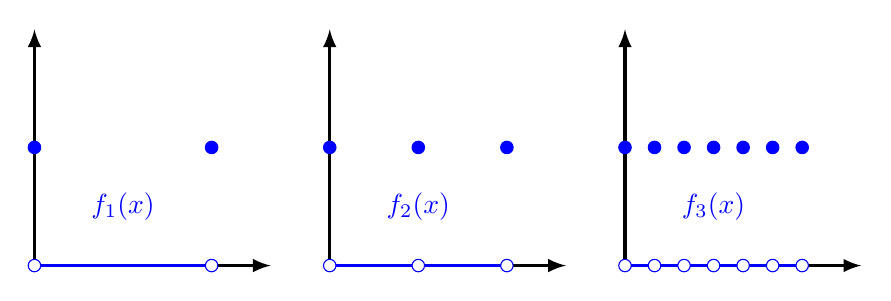
\begin{tikzpicture}[scale = 1.5]
        \draw[-latex, very thick] (0, 0) -- (0, 2);
        \draw[-latex, very thick] (0, 0) -- (2, 0);
        \draw[-latex, very thick] (2.5, 0) -- (2.5, 2);
        \draw[-latex, very thick] (2.5, 0) -- (4.5, 0);
        \draw[-latex, very thick] (5, 0) -- (5, 2);
        \draw[-latex, very thick] (5, 0) -- (7, 0);
        \filldraw[blue] (0, 1) circle (1.5pt);
        \filldraw[blue] (1.5, 1) circle (1.5pt);
        \draw[thick, blue] (0, 0) -- (1.5, 0);
        \draw[blue, fill = white] (0, 0) circle (1.5pt);
        \draw[blue, fill = white] (1.5, 0) circle (1.5pt);
        \node[text = blue] at (0.75, 0.5) {$f_1(x)$};

        \filldraw[blue] (2.5, 1) circle (1.5pt);
        \filldraw[blue] (3.25, 1) circle (1.5pt);
        \filldraw[blue] (4, 1) circle (1.5pt);
        \draw[thick, blue] (2.5, 0) -- (4, 0);
        \draw[blue, fill = white] (2.5, 0) circle (1.5pt);
        \draw[blue, fill = white] (3.25, 0) circle (1.5pt);
        \draw[blue, fill = white] (4, 0) circle (1.5pt);
        \node[text = blue] at (3.25, 0.5) {$f_2(x)$};

        \filldraw[blue] (5, 1) circle (1.5pt);
        \filldraw[blue] (5.25, 1) circle (1.5pt);
        \filldraw[blue] (5.5, 1) circle (1.5pt);
        \filldraw[blue] (5.75, 1) circle (1.5pt);
        \filldraw[blue] (6, 1) circle (1.5pt);
        \filldraw[blue] (6.25, 1) circle (1.5pt);
        \filldraw[blue] (6.5, 1) circle (1.5pt);
        \draw[thick, blue] (5, 0) -- (6.5, 0);
        \draw[blue, fill = white] (5, 0) circle (1.5pt);
        \draw[blue, fill = white] (5.25, 0) circle (1.5pt);
        \draw[blue, fill = white] (5.5, 0) circle (1.5pt);
        \draw[blue, fill = white] (5.75, 0) circle (1.5pt);
        \draw[blue, fill = white] (6, 0) circle (1.5pt);
        \draw[blue, fill = white] (6.25, 0) circle (1.5pt);
        \draw[blue, fill = white] (6.5, 0) circle (1.5pt);
        \node[text = blue] at (5.75, 0.5) {$f_3(x)$};
    \end{tikzpicture}
    \caption{Plot of $f_m(x)$ over the interval $[0, 1]$ for $m = 1, 2, 3$. For $m = 1$, only $x = 0, 1$ satisfy $m! x = x \in \ZZ$. For $m = 2$, we have that $x = 0, \frac{1}{2}, 1$ satisfy $m!x = 2x \in \ZZ$. Finally, for $m = 3$, we have that $x = 0, \frac{1}{6}, \frac{2}{6}, \frac{3}{6}, \frac{4}{6}, \frac{5}{6}, 1$ satisfy $m!x = 6x \in \ZZ$.}
    \label{fig38}
\end{figure}

\noindent We now show that $f$ defined in the above example is not Riemann integrable on $[0, 1]$.

\begin{proof}
    Consider any partition $P$ of $[0, 1]$. Due to the density of rational and irrational numbers in $\RR$ (Theorem \ref{thm:1.20}) we have that $M_i = \sup{f(x): x \in [x_{i-1}, x_i]} = 1$ and $m_i = \inf{f(x): x \in [x_{i-1}, x_i]} = 0$ for all $i$. Therefore, we have that $U(P, f) = \sum_{i=1}^N M_i \Delta x_i = 1$ and $L(P, f) = \sum_{i=1}^N m_i \Delta x_i = 0$ for all partitions $P$. Therefore, $\sup_P U(P, f) = 1$ and $\inf_P L(P, f) = 0$, and we conclude that $f$ is not Riemann integrable on $[0, 1]$.
\end{proof}


\begin{nexample}{}{}
    Define $f_n$ such that:
    \begin{align*}
        f_n(x) = \begin{cases}
            0 & \abs{x} \geq \frac{1}{n}
            \\ n(nx+1) & -\frac{1}{n} < x < 0
            \\ -n(nx+1) & 0 < x < \frac{1}{n}
            \\ 0 & x = 0
        \end{cases}
    \end{align*}
    Then, we have that $f(x) = \linf f_n(x) = 0$ for all $x$.  Furthermore, we have that $\int_{-1}^1 f_n(x)dx = 1$ for all $n$, but $\int_{-1}^1 f(x)dx = 0$. Hence, we have that:
    \begin{align*}
        \linf \int_{-1}^1 f_n(x)dx = 1 \neq 0 = \int_{-1}^1 \linf f_n(x) dx
    \end{align*}
    showing that problems can arise when we interchange the order of an integral with a limit.
\end{nexample}

\begin{figure}[htbp]
    \centering
    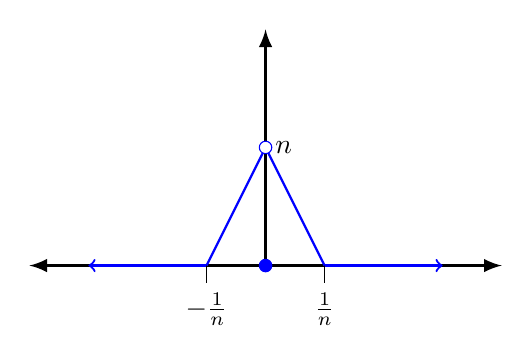
\begin{tikzpicture}[scale=1.5]
        \draw[latex-latex, very thick] (-2, 0) -- (2, 0);
        \draw[-latex , very thick] (0, 0) -- (0, 2);
        \draw[<-, thick, blue] (-1.5, 0) -- (-0.5, 0);
        \draw[thick, blue] (-0.5, 0) -- (0, 1);
        \draw[thick, blue] (0, 1) -- (0.5, 0);
        \draw[->, thick, blue] (0.5, 0) -- (1.5, 0);
        \filldraw[blue] (0, 0) circle (1.5pt);
        \draw[blue, fill = white] (0, 1) circle (1.5pt);
        \node[right] at (0, 1) {$n$};
        \draw[] (-0.5, 0) -- (-0.5, -0.15);
        \node[below] at (-0.5, -0.15) {$-\frac{1}{n}$};
        \draw[] (0.5, 0) -- (0.5, -0.15);
        \node[below] at (0.5, -0.15) {$\frac{1}{n}$};
    \end{tikzpicture}
    
    \caption{Plot of $f_n$ in the above example.}
    \label{fig39}
\end{figure}

\begin{example}{}{7.5}
    Let $f_n(x) = \frac{\sin nx}{\sqrt{n}}$ for $n \in \NN, x \in \RR$. Then, let $f(x) = \linf f_n(x) = 0$ for all $x \in \RR$, so $f'(x) = 0$. However, $f'_n(x) = \frac{1}{\sqrt{n}}n \cos n x = \sqrt{n} \cos n x$ and $\linf \sqrt{n} \cos n x$ does not exist. For example, $f_n'(\pi) = \sqrt{n}(-1)^n$ which is a divergent sequence. So:
    \begin{align*}
        f'(\pi) = \left(\linf f_n\right)'(\pi) = 0 \neq \linf f_n'(\pi)
    \end{align*}
    whcih shows us that problems can arise when interchanging a derivative (which is just a type of limit) with a limit.
\end{example}
\noindent With the above five examples, we have seen examples of bad behaviour that can occur under interchange of limits. Namely:
\begin{enumerate}[1.]
    \item An interchange of the order of limits can change the limiting value for a double sequence.
    \item The limit of a sequence of continuous functions is not necessarily continuous.
    \item The limit of a sequence of Riemann integrable functions is not necessarily Riemann integrable.
    \item The limit of a sequence of Riemann integrals can differ from the Riemann integral of the limit of a sequence.
    \item The limit of a sequence of derivatives can differ from the derivative of a limit of a sequence.
\end{enumerate}

\noindent The good news is that in all of these examples, the sequences we looked at had a ``weak'' form of convergence, where we fix $x$ and then take the $n \rightarrow \infty$ limit. We will now proceed to look at a stronger version of convergence, which looks at ``all $x$ at once'', ensuring that this bad behaviour does not (for the most part) occur.

\subsection{Uniform Convergence}

\setcounter{rudin}{6}
\begin{definition}{Uniform Convergence}{7.7}
    Let $E$ be any set and $f_n: E \mapsto \RR$ or $f_n: E \mapsto \CC$ for $n \in \NN$. Then, $f_n$ \textbf{converges uniformly} to $f$ on $E$ if for all $\e > 0$, there exists $N$ such that $n \geq N$ implies that $\abs{f_n(x) - f(x)} < \e$ for all $x \in E$. 
\end{definition}
\noindent Note the lack of $x$ dependence in the above definition. We give a useful visual intuition of uniform convergence below:

\begin{figure}[htbp]
    \centering
    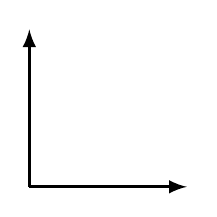
\begin{tikzpicture}
        \draw[-latex, very thick] (0, 0) -- (2, 0);
        \draw[-latex, very thick] (0, 0) -- (0, 2);
    \end{tikzpicture}
    
    \caption{Visualization of uniform convergence. If $f_n \rightarrow f$, uniformly, for any $\e > 0$, we can find $N$ such that for $n \geq N$, $f_n(x)$ lies in the $\e$-tube around $f$.}
    \label{fig40}
\end{figure}

\begin{nexample}{}{}
    
\end{nexample}

\begin{nexample}{}{}
    
\end{nexample}

\begin{theorem}{Cauchy Criterion for Uniform Convergence}{7.8}
    
\end{theorem}
\begin{nproof}
    
\end{nproof}

\begin{theorem}{}{7.9}
    
\end{theorem}
\begin{nproof}
    
\end{nproof}

\begin{ndef}{: Uniform Convergence of Series}{}
    
\end{ndef}

\begin{theorem}{Weierstrauss M-Test}{7.10}
    
\end{theorem}
\begin{nproof}
    
\end{nproof}

\subsection{Uniform Convergence and Integration}

\subsection{Uniform Convergence and Differentiation}

\subsection{Equicontinuituous Families of Functions}

\subsection{The Stone-Weierstrauss Theorem}

